\chapter{Implementacja projektu}

Projekt `Planning poker', to aplikacja webową opartą o platformę Firebase,
która jest napisana przy użyciu bibliotek React.js w programie visual studio code.
Aby zachować porządek i możliwość późniejszego rozwoju aplikacji o nowe komponenty,
koniecznym jest stworzenie uporządkowanej struktury plików zawartych w projekcie.
~rys.\ref{rys:projekt}
\begin{figure}
	\centering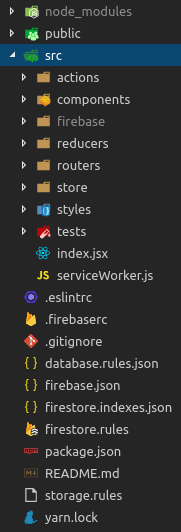
\includegraphics[width=.3\textwidth]{img/projekt}
	\caption{Struktura projektu}\label{rys:projekt}% Źródło rysunku i etykieta przez którą odwołujemy się do rysunku.
\end{figure}
Folderem zawierającym wszystkie podfoldery oraz pliki jest folder `scrumpoker' (jest to druga wersja aplikacji).
Pliki takie jak `storage.rules' czy `.firebaesrc' powstały automatycznie w procesie konfiguracji usługi firebase.
Plik `package.json' zabiera całą konfigurację projetku stworzonego dzięki narzędziu `create-react-app'.
Folder `node modules' zawiera zawiera zależności, niezbędne do uruchomienia aplikacji.
    Folder src zawiera cały kod aplikacji. Jest on najważniejszy w całym projekcie.
Głównym plikiem projektu jest `index.jsx'. To w tym pliku renderowana jest cała aplikacja.
Aby uruchomić program niezbędny jest też backend w postaci utworzonego i skonfigurowanego projektu firebase.
Konfiguracje należy umieścić w pliku `src/firebase/firebase.jsx'. Listing:
~\ref{listing:firebaseConfig} 

\begin{listing}
	\begin{minted}{c}
import * as firebase from 'firebase';

var config = {
    apiKey: "<API_KEY>",
    authDomain: "<PROJECT_ID>.firebaseapp.com",
    databaseURL: "https://<DATABASE_NAME>.firebaseio.com",
    projectId: "<PROJECT_ID>",
    storageBucket: "<BUCKET>.appspot.com",
    messagingSenderId: "<SENDER_ID>",
  };

firebase.initializeApp(config);

const database = firebase.firestore();
const settings = { timestampsInSnapshots: true};
database.settings(settings);
export { firebase, database as default };
	\end{minted}
	\caption{Konfiguracja firebase} \label{listing:firebaseConfig}
\end{listing}